% Options for packages loaded elsewhere
\PassOptionsToPackage{unicode}{hyperref}
\PassOptionsToPackage{hyphens}{url}
%
\documentclass[
]{article}
\usepackage{amsmath,amssymb}
\usepackage{iftex}
\ifPDFTeX
  \usepackage[T1]{fontenc}
  \usepackage[utf8]{inputenc}
  \usepackage{textcomp} % provide euro and other symbols
\else % if luatex or xetex
  \usepackage{unicode-math} % this also loads fontspec
  \defaultfontfeatures{Scale=MatchLowercase}
  \defaultfontfeatures[\rmfamily]{Ligatures=TeX,Scale=1}
\fi
\usepackage{lmodern}
\ifPDFTeX\else
  % xetex/luatex font selection
\fi
% Use upquote if available, for straight quotes in verbatim environments
\IfFileExists{upquote.sty}{\usepackage{upquote}}{}
\IfFileExists{microtype.sty}{% use microtype if available
  \usepackage[]{microtype}
  \UseMicrotypeSet[protrusion]{basicmath} % disable protrusion for tt fonts
}{}
\makeatletter
\@ifundefined{KOMAClassName}{% if non-KOMA class
  \IfFileExists{parskip.sty}{%
    \usepackage{parskip}
  }{% else
    \setlength{\parindent}{0pt}
    \setlength{\parskip}{6pt plus 2pt minus 1pt}}
}{% if KOMA class
  \KOMAoptions{parskip=half}}
\makeatother
\usepackage{xcolor}
\usepackage[margin=1in]{geometry}
\usepackage{color}
\usepackage{fancyvrb}
\newcommand{\VerbBar}{|}
\newcommand{\VERB}{\Verb[commandchars=\\\{\}]}
\DefineVerbatimEnvironment{Highlighting}{Verbatim}{commandchars=\\\{\}}
% Add ',fontsize=\small' for more characters per line
\usepackage{framed}
\definecolor{shadecolor}{RGB}{248,248,248}
\newenvironment{Shaded}{\begin{snugshade}}{\end{snugshade}}
\newcommand{\AlertTok}[1]{\textcolor[rgb]{0.94,0.16,0.16}{#1}}
\newcommand{\AnnotationTok}[1]{\textcolor[rgb]{0.56,0.35,0.01}{\textbf{\textit{#1}}}}
\newcommand{\AttributeTok}[1]{\textcolor[rgb]{0.13,0.29,0.53}{#1}}
\newcommand{\BaseNTok}[1]{\textcolor[rgb]{0.00,0.00,0.81}{#1}}
\newcommand{\BuiltInTok}[1]{#1}
\newcommand{\CharTok}[1]{\textcolor[rgb]{0.31,0.60,0.02}{#1}}
\newcommand{\CommentTok}[1]{\textcolor[rgb]{0.56,0.35,0.01}{\textit{#1}}}
\newcommand{\CommentVarTok}[1]{\textcolor[rgb]{0.56,0.35,0.01}{\textbf{\textit{#1}}}}
\newcommand{\ConstantTok}[1]{\textcolor[rgb]{0.56,0.35,0.01}{#1}}
\newcommand{\ControlFlowTok}[1]{\textcolor[rgb]{0.13,0.29,0.53}{\textbf{#1}}}
\newcommand{\DataTypeTok}[1]{\textcolor[rgb]{0.13,0.29,0.53}{#1}}
\newcommand{\DecValTok}[1]{\textcolor[rgb]{0.00,0.00,0.81}{#1}}
\newcommand{\DocumentationTok}[1]{\textcolor[rgb]{0.56,0.35,0.01}{\textbf{\textit{#1}}}}
\newcommand{\ErrorTok}[1]{\textcolor[rgb]{0.64,0.00,0.00}{\textbf{#1}}}
\newcommand{\ExtensionTok}[1]{#1}
\newcommand{\FloatTok}[1]{\textcolor[rgb]{0.00,0.00,0.81}{#1}}
\newcommand{\FunctionTok}[1]{\textcolor[rgb]{0.13,0.29,0.53}{\textbf{#1}}}
\newcommand{\ImportTok}[1]{#1}
\newcommand{\InformationTok}[1]{\textcolor[rgb]{0.56,0.35,0.01}{\textbf{\textit{#1}}}}
\newcommand{\KeywordTok}[1]{\textcolor[rgb]{0.13,0.29,0.53}{\textbf{#1}}}
\newcommand{\NormalTok}[1]{#1}
\newcommand{\OperatorTok}[1]{\textcolor[rgb]{0.81,0.36,0.00}{\textbf{#1}}}
\newcommand{\OtherTok}[1]{\textcolor[rgb]{0.56,0.35,0.01}{#1}}
\newcommand{\PreprocessorTok}[1]{\textcolor[rgb]{0.56,0.35,0.01}{\textit{#1}}}
\newcommand{\RegionMarkerTok}[1]{#1}
\newcommand{\SpecialCharTok}[1]{\textcolor[rgb]{0.81,0.36,0.00}{\textbf{#1}}}
\newcommand{\SpecialStringTok}[1]{\textcolor[rgb]{0.31,0.60,0.02}{#1}}
\newcommand{\StringTok}[1]{\textcolor[rgb]{0.31,0.60,0.02}{#1}}
\newcommand{\VariableTok}[1]{\textcolor[rgb]{0.00,0.00,0.00}{#1}}
\newcommand{\VerbatimStringTok}[1]{\textcolor[rgb]{0.31,0.60,0.02}{#1}}
\newcommand{\WarningTok}[1]{\textcolor[rgb]{0.56,0.35,0.01}{\textbf{\textit{#1}}}}
\usepackage{graphicx}
\makeatletter
\newsavebox\pandoc@box
\newcommand*\pandocbounded[1]{% scales image to fit in text height/width
  \sbox\pandoc@box{#1}%
  \Gscale@div\@tempa{\textheight}{\dimexpr\ht\pandoc@box+\dp\pandoc@box\relax}%
  \Gscale@div\@tempb{\linewidth}{\wd\pandoc@box}%
  \ifdim\@tempb\p@<\@tempa\p@\let\@tempa\@tempb\fi% select the smaller of both
  \ifdim\@tempa\p@<\p@\scalebox{\@tempa}{\usebox\pandoc@box}%
  \else\usebox{\pandoc@box}%
  \fi%
}
% Set default figure placement to htbp
\def\fps@figure{htbp}
\makeatother
\setlength{\emergencystretch}{3em} % prevent overfull lines
\providecommand{\tightlist}{%
  \setlength{\itemsep}{0pt}\setlength{\parskip}{0pt}}
\setcounter{secnumdepth}{-\maxdimen} % remove section numbering
\usepackage{ctex}
\usepackage{bookmark}
\IfFileExists{xurl.sty}{\usepackage{xurl}}{} % add URL line breaks if available
\urlstyle{same}
\hypersetup{
  pdftitle={WK11\_2022\_23},
  hidelinks,
  pdfcreator={LaTeX via pandoc}}

\title{WK11\_2022\_23}
\author{}
\date{\vspace{-2.5em}2025-09-09}

\begin{document}
\maketitle

\begin{Shaded}
\begin{Highlighting}[]
\FunctionTok{library}\NormalTok{(tidyverse)}
\end{Highlighting}
\end{Shaded}

\begin{verbatim}
## -- Attaching core tidyverse packages ------------------------ tidyverse 2.0.0 --
## v dplyr     1.1.4     v readr     2.1.5
## v forcats   1.0.0     v stringr   1.5.1
## v ggplot2   3.5.2     v tibble    3.2.1
## v lubridate 1.9.4     v tidyr     1.3.1
## v purrr     1.0.4     
## -- Conflicts ------------------------------------------ tidyverse_conflicts() --
## x dplyr::filter() masks stats::filter()
## x dplyr::lag()    masks stats::lag()
## i Use the conflicted package (<http://conflicted.r-lib.org/>) to force all conflicts to become errors
\end{verbatim}

\begin{Shaded}
\begin{Highlighting}[]
\FunctionTok{library}\NormalTok{(readxl)}
\FunctionTok{library}\NormalTok{(lubridate)}
\FunctionTok{library}\NormalTok{(janitor)}
\end{Highlighting}
\end{Shaded}

\begin{verbatim}
## 
## Attaching package: 'janitor'
## 
## The following objects are masked from 'package:stats':
## 
##     chisq.test, fisher.test
\end{verbatim}

\begin{Shaded}
\begin{Highlighting}[]
\FunctionTok{library}\NormalTok{(purrr)}
\FunctionTok{library}\NormalTok{(readr)}
\FunctionTok{library}\NormalTok{(ggthemes)}
\FunctionTok{library}\NormalTok{(ggeffects)}
\FunctionTok{library}\NormalTok{(lme4)}
\end{Highlighting}
\end{Shaded}

\begin{verbatim}
## Loading required package: Matrix
## 
## Attaching package: 'Matrix'
## 
## The following objects are masked from 'package:tidyr':
## 
##     expand, pack, unpack
\end{verbatim}

\begin{Shaded}
\begin{Highlighting}[]
\FunctionTok{library}\NormalTok{(dplyr)}
\FunctionTok{library}\NormalTok{(ggplot2)}
\FunctionTok{library}\NormalTok{(emmeans)      }
\end{Highlighting}
\end{Shaded}

\begin{verbatim}
## Welcome to emmeans.
## Caution: You lose important information if you filter this package's results.
## See '? untidy'
\end{verbatim}

\begin{Shaded}
\begin{Highlighting}[]
\FunctionTok{library}\NormalTok{(broom.mixed)  }
\FunctionTok{library}\NormalTok{(viridis)      }
\end{Highlighting}
\end{Shaded}

\begin{verbatim}
## Loading required package: viridisLite
\end{verbatim}

\begin{Shaded}
\begin{Highlighting}[]
\FunctionTok{library}\NormalTok{(nlme)         }
\end{Highlighting}
\end{Shaded}

\begin{verbatim}
## 
## Attaching package: 'nlme'
## 
## The following object is masked from 'package:lme4':
## 
##     lmList
## 
## The following object is masked from 'package:dplyr':
## 
##     collapse
\end{verbatim}

\begin{Shaded}
\begin{Highlighting}[]
\FunctionTok{library}\NormalTok{(mgcv)         }
\end{Highlighting}
\end{Shaded}

\begin{verbatim}
## This is mgcv 1.9-3. For overview type 'help("mgcv-package")'.
\end{verbatim}

\begin{Shaded}
\begin{Highlighting}[]
\FunctionTok{setwd}\NormalTok{(}\StringTok{"C:/Users/Tobyz/Desktop/Toby在大学/Maloof Lab/S.tort{-}light{-}growth/Data"}\NormalTok{)}
\end{Highlighting}
\end{Shaded}

\emph{import plant data}

\begin{Shaded}
\begin{Highlighting}[]
\NormalTok{plant\_2223 }\OtherTok{\textless{}{-}} \FunctionTok{read.csv}\NormalTok{(}\StringTok{"C:/Users/Tobyz/Desktop/Toby在大学/Maloof Lab/S.tort{-}light{-}growth/Data/UCD\_2022\_23\_size\_data\_combined.csv"}\NormalTok{) }\SpecialCharTok{\%\textgreater{}\%}
  \FunctionTok{clean\_names}\NormalTok{() }\SpecialCharTok{\%\textgreater{}\%}
  \FunctionTok{mutate}\NormalTok{(}\AttributeTok{survey\_date =} \FunctionTok{as.Date}\NormalTok{(survey\_date, }\AttributeTok{format =} \StringTok{"\%m/\%d/\%Y"}\NormalTok{))}
\FunctionTok{summary}\NormalTok{(plant\_2223)}
\end{Highlighting}
\end{Shaded}

\begin{verbatim}
##   survey_date            block                row            col           
##  Min.   :2023-01-27   Length:13626       Min.   : 3.00   Length:13626      
##  1st Qu.:2023-03-17   Class :character   1st Qu.:12.00   Class :character  
##  Median :2023-04-20   Mode  :character   Median :22.00   Mode  :character  
##  Mean   :2023-04-26                      Mean   :21.84                     
##  3rd Qu.:2023-06-12                      3rd Qu.:32.00                     
##  Max.   :2023-07-24                      Max.   :42.00                     
##                                                                            
##      pop                  mf              rep              height       
##  Length:13626       Min.   : 1.000   Min.   :  1.000   Min.   :  0.100  
##  Class :character   1st Qu.: 2.000   1st Qu.:  4.000   1st Qu.:  2.300  
##  Mode  :character   Median : 4.000   Median :  8.000   Median :  3.850  
##                     Mean   : 4.363   Mean   :  8.753   Mean   :  9.836  
##                     3rd Qu.: 6.000   3rd Qu.: 12.000   3rd Qu.:  7.700  
##                     Max.   :12.000   Max.   :100.000   Max.   :130.000  
##                     NA's   :2        NA's   :2         NA's   :10542    
##   longest_leaf   
##  Min.   : 0.000  
##  1st Qu.: 2.100  
##  Median : 3.200  
##  Mean   : 3.827  
##  3rd Qu.: 5.200  
##  Max.   :12.700  
##  NA's   :10551
\end{verbatim}

\emph{import light data}

\begin{Shaded}
\begin{Highlighting}[]
\NormalTok{light\_raw\_2223 }\OtherTok{\textless{}{-}} \FunctionTok{read\_csv}\NormalTok{(}\StringTok{"C:/Users/Tobyz/Desktop/Toby在大学/Maloof Lab/S.tort{-}light{-}growth/Data/UCD\_met\_data.csv"}\NormalTok{)}\SpecialCharTok{\%\textgreater{}\%}\FunctionTok{clean\_names}\NormalTok{()}\SpecialCharTok{\%\textgreater{}\%}
 \FunctionTok{mutate}\NormalTok{(}
    \AttributeTok{date =} \FunctionTok{mdy}\NormalTok{(date),}
    \AttributeTok{sol\_rad\_ly\_day =} \FunctionTok{as.numeric}\NormalTok{(sol\_rad\_ly\_day),  }\CommentTok{\# turn into number format}
\NormalTok{  )}
\end{Highlighting}
\end{Shaded}

\begin{verbatim}
## New names:
## Rows: 188 Columns: 33
## -- Column specification
## -------------------------------------------------------- Delimiter: "," chr
## (17): Stn Name, CIMIS Region, Date, Jul, qc...9, qc...11, qc...13, qc...... dbl
## (15): Stn Id, ETo (in), Precip (in), Sol Rad (Ly/day), Avg Vap Pres (mBa... lgl
## (1): qc...7
## i Use `spec()` to retrieve the full column specification for this data. i
## Specify the column types or set `show_col_types = FALSE` to quiet this message.
## * `qc` -> `qc...7`
## * `qc` -> `qc...9`
## * `qc` -> `qc...11`
## * `qc` -> `qc...13`
## * `qc` -> `qc...15`
## * `qc` -> `qc...17`
## * `qc` -> `qc...19`
## * `qc` -> `qc...21`
## * `qc` -> `qc...23`
## * `qc` -> `qc...25`
## * `qc` -> `qc...27`
## * `qc` -> `qc...29`
## * `qc` -> `qc...31`
## * `qc` -> `qc...33`
\end{verbatim}

\emph{Investigate or filter out plants that show negative growth} \#Q:
How could we deal with bad observations? \#Solution: find out tolerance
value and then filter out observance data lager than the tolerance value
\#Figure A: Histogram showing the frequency of decreases in plant height
between consecutive surveys. Most negative growth values are close to
zero, likely reflecting measurement noise, while a small number of
extreme decreases (\textless=--5 cm) suggest errors and were removed
from subsequent analyses.

\begin{Shaded}
\begin{Highlighting}[]
\CommentTok{\#PID}
\NormalTok{pl\_gr }\OtherTok{\textless{}{-}}\NormalTok{ plant\_2223 }\SpecialCharTok{\%\textgreater{}\%}
  \FunctionTok{unite}\NormalTok{(}\StringTok{"PID"}\NormalTok{, pop}\SpecialCharTok{:}\NormalTok{rep, }\AttributeTok{sep =} \StringTok{"\_"}\NormalTok{, }\AttributeTok{remove =} \ConstantTok{FALSE}\NormalTok{) }\SpecialCharTok{\%\textgreater{}\%}
  \FunctionTok{mutate}\NormalTok{(}\AttributeTok{survey\_date =} \FunctionTok{as.Date}\NormalTok{(survey\_date))}

\CommentTok{\#find out plants with negative growth}
\NormalTok{pl\_gr }\SpecialCharTok{\%\textgreater{}\%}
  \FunctionTok{arrange}\NormalTok{(PID, survey\_date) }\SpecialCharTok{\%\textgreater{}\%}  \CommentTok{\# arrange in time sequence}
  \FunctionTok{group\_by}\NormalTok{(PID) }\SpecialCharTok{\%\textgreater{}\%}
  \FunctionTok{mutate}\NormalTok{(}\AttributeTok{growth =}\NormalTok{ height }\SpecialCharTok{{-}} \FunctionTok{lag}\NormalTok{(height)) }\SpecialCharTok{\%\textgreater{}\%}  \CommentTok{\# find out the diff btw nearby dates}
  \FunctionTok{summarise}\NormalTok{(}\AttributeTok{has\_negative\_growth =} \FunctionTok{any}\NormalTok{(growth }\SpecialCharTok{\textless{}} \DecValTok{0}\NormalTok{, }\AttributeTok{na.rm =} \ConstantTok{TRUE}\NormalTok{)) }\SpecialCharTok{\%\textgreater{}\%} 
  \FunctionTok{filter}\NormalTok{(has\_negative\_growth) }\OtherTok{{-}\textgreater{}}\NormalTok{ neg\_gr\_pl}
\NormalTok{neg\_gr\_pl}
\end{Highlighting}
\end{Shaded}

\begin{verbatim}
## # A tibble: 453 x 2
##    PID     has_negative_growth
##    <chr>   <lgl>              
##  1 BH_1_10 TRUE               
##  2 BH_1_7  TRUE               
##  3 BH_1_8  TRUE               
##  4 BH_2_1  TRUE               
##  5 BH_2_10 TRUE               
##  6 BH_2_11 TRUE               
##  7 BH_2_12 TRUE               
##  8 BH_2_13 TRUE               
##  9 BH_2_14 TRUE               
## 10 BH_2_3  TRUE               
## # i 443 more rows
\end{verbatim}

\begin{Shaded}
\begin{Highlighting}[]
\CommentTok{\#find out tolerance value}
\NormalTok{neg\_gr\_v }\OtherTok{\textless{}{-}}\NormalTok{ pl\_gr }\SpecialCharTok{\%\textgreater{}\%}
  \FunctionTok{arrange}\NormalTok{(PID, survey\_date) }\SpecialCharTok{\%\textgreater{}\%}
  \FunctionTok{group\_by}\NormalTok{(PID) }\SpecialCharTok{\%\textgreater{}\%}
  \FunctionTok{mutate}\NormalTok{(}\AttributeTok{growth =}\NormalTok{ height }\SpecialCharTok{{-}} \FunctionTok{lag}\NormalTok{(height)) }\SpecialCharTok{\%\textgreater{}\%}
  \FunctionTok{ungroup}\NormalTok{() }\SpecialCharTok{\%\textgreater{}\%}
  \FunctionTok{filter}\NormalTok{(growth }\SpecialCharTok{\textless{}} \DecValTok{0}\NormalTok{)}

\FunctionTok{ggplot}\NormalTok{(neg\_gr\_v, }\FunctionTok{aes}\NormalTok{(}\AttributeTok{x =}\NormalTok{ growth)) }\SpecialCharTok{+}
  \FunctionTok{geom\_histogram}\NormalTok{(}\AttributeTok{binwidth =} \FloatTok{0.5}\NormalTok{, }\AttributeTok{fill =} \StringTok{"red"}\NormalTok{, }\AttributeTok{color =} \StringTok{"black"}\NormalTok{) }\SpecialCharTok{+}
  \FunctionTok{labs}\NormalTok{(}
    \AttributeTok{title =} \StringTok{"Figure A: Distribution of Negative Growth Values"}\NormalTok{,}
    \AttributeTok{x =} \StringTok{"Height Decrease (cm)"}\NormalTok{,}
    \AttributeTok{y =} \StringTok{"Count"}
\NormalTok{  ) }\SpecialCharTok{+}
  \FunctionTok{theme\_bw}\NormalTok{()}
\end{Highlighting}
\end{Shaded}

\pandocbounded{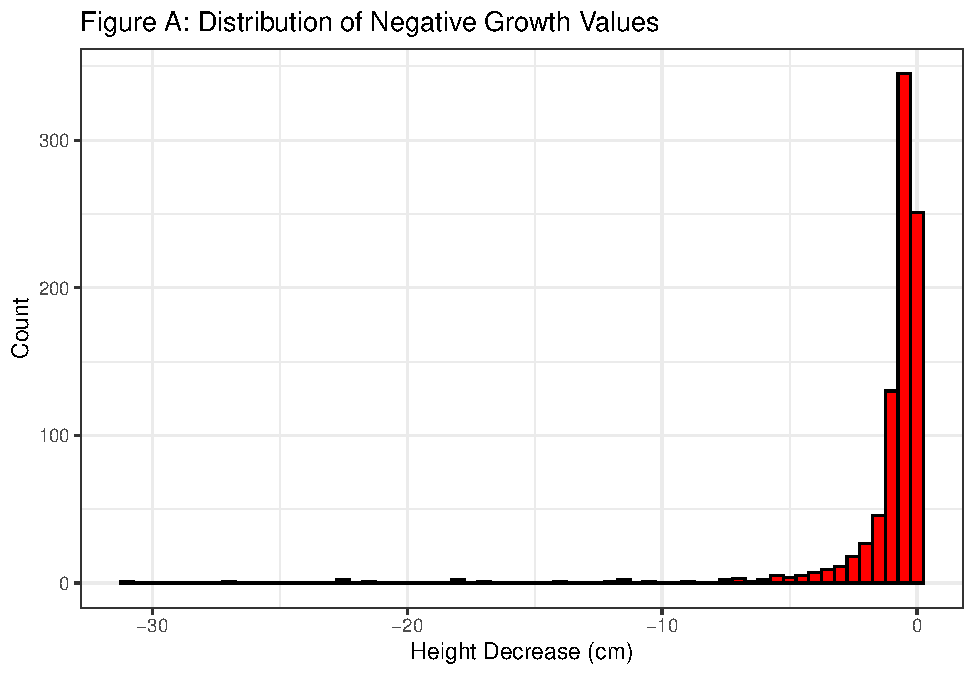
\includegraphics[keepaspectratio]{WK11_2022_23_files/figure-latex/unnamed-chunk-4-1.pdf}}

\begin{Shaded}
\begin{Highlighting}[]
\CommentTok{\#filter out plants with negative growth \textless{} {-}5}
\NormalTok{pl\_gr\_cleaned }\OtherTok{\textless{}{-}}\NormalTok{ pl\_gr}

\ControlFlowTok{repeat}\NormalTok{ \{}
\NormalTok{  pl\_gr\_cleaned }\OtherTok{\textless{}{-}}\NormalTok{ pl\_gr\_cleaned }\SpecialCharTok{\%\textgreater{}\%}
    \FunctionTok{arrange}\NormalTok{(PID, survey\_date) }\SpecialCharTok{\%\textgreater{}\%}
    \FunctionTok{group\_by}\NormalTok{(PID) }\SpecialCharTok{\%\textgreater{}\%}
    \FunctionTok{mutate}\NormalTok{(}\AttributeTok{growth =}\NormalTok{ height }\SpecialCharTok{{-}} \FunctionTok{lag}\NormalTok{(height)) }\SpecialCharTok{\%\textgreater{}\%}
    \FunctionTok{filter}\NormalTok{(}\FunctionTok{is.na}\NormalTok{(growth) }\SpecialCharTok{|}\NormalTok{ growth }\SpecialCharTok{\textgreater{}=} \SpecialCharTok{{-}}\DecValTok{5}\NormalTok{) }\SpecialCharTok{\%\textgreater{}\%}
    \FunctionTok{select}\NormalTok{(}\SpecialCharTok{{-}}\NormalTok{growth) }\SpecialCharTok{\%\textgreater{}\%}
    \FunctionTok{ungroup}\NormalTok{()}

\NormalTok{  check }\OtherTok{\textless{}{-}}\NormalTok{ pl\_gr\_cleaned }\SpecialCharTok{\%\textgreater{}\%}
    \FunctionTok{arrange}\NormalTok{(PID, survey\_date) }\SpecialCharTok{\%\textgreater{}\%}
    \FunctionTok{group\_by}\NormalTok{(PID) }\SpecialCharTok{\%\textgreater{}\%}
    \FunctionTok{mutate}\NormalTok{(}\AttributeTok{growth =}\NormalTok{ height }\SpecialCharTok{{-}} \FunctionTok{lag}\NormalTok{(height)) }\SpecialCharTok{\%\textgreater{}\%}
    \FunctionTok{filter}\NormalTok{(growth }\SpecialCharTok{\textless{}} \SpecialCharTok{{-}}\DecValTok{5}\NormalTok{)}
  
  \ControlFlowTok{if}\NormalTok{ (}\FunctionTok{nrow}\NormalTok{(check) }\SpecialCharTok{==} \DecValTok{0}\NormalTok{) }\ControlFlowTok{break}
\NormalTok{\}}
\end{Highlighting}
\end{Shaded}

\emph{Measure Growth via Daily Growth Rate}

\begin{Shaded}
\begin{Highlighting}[]
\CommentTok{\#define daily growth rate}
\NormalTok{pl\_gr\_daily }\OtherTok{\textless{}{-}}\NormalTok{ pl\_gr\_cleaned }\SpecialCharTok{\%\textgreater{}\%}
  \FunctionTok{arrange}\NormalTok{(PID, survey\_date) }\SpecialCharTok{\%\textgreater{}\%}
  \FunctionTok{group\_by}\NormalTok{(PID) }\SpecialCharTok{\%\textgreater{}\%}
  \FunctionTok{mutate}\NormalTok{(}
    \AttributeTok{prev\_height =} \FunctionTok{lag}\NormalTok{(height),}
    \AttributeTok{prev\_date =} \FunctionTok{lag}\NormalTok{(survey\_date),}
    \AttributeTok{days\_elapsed =} \FunctionTok{as.numeric}\NormalTok{(survey\_date }\SpecialCharTok{{-}}\NormalTok{ prev\_date),}
    \AttributeTok{daily\_growth =}\NormalTok{ (height }\SpecialCharTok{{-}}\NormalTok{ prev\_height) }\SpecialCharTok{/}\NormalTok{ days\_elapsed}
\NormalTok{  ) }\SpecialCharTok{\%\textgreater{}\%}
  \FunctionTok{ungroup}\NormalTok{()}
\end{Highlighting}
\end{Shaded}

\emph{Calculate Daily Mean Solar Radiation}

\begin{Shaded}
\begin{Highlighting}[]
\NormalTok{pl\_lt }\OtherTok{\textless{}{-}}\NormalTok{ pl\_gr\_daily }\SpecialCharTok{\%\textgreater{}\%}
  \FunctionTok{rowwise}\NormalTok{() }\SpecialCharTok{\%\textgreater{}\%}
  \FunctionTok{mutate}\NormalTok{(}
    \AttributeTok{mean\_light\_ly\_day =} \FunctionTok{mean}\NormalTok{(}
\NormalTok{      light\_raw\_2223}\SpecialCharTok{$}\NormalTok{sol\_rad\_ly\_day[}
        \SpecialCharTok{!}\FunctionTok{is.na}\NormalTok{(light\_raw\_2223}\SpecialCharTok{$}\NormalTok{date) }\SpecialCharTok{\&}
\NormalTok{        light\_raw\_2223}\SpecialCharTok{$}\NormalTok{date }\SpecialCharTok{\textgreater{}}\NormalTok{ prev\_date }\SpecialCharTok{\&}
\NormalTok{        light\_raw\_2223}\SpecialCharTok{$}\NormalTok{date }\SpecialCharTok{\textless{}=}\NormalTok{ survey\_date}
\NormalTok{      ],}
      \AttributeTok{na.rm =} \ConstantTok{TRUE}
\NormalTok{    ),}
    \AttributeTok{n\_days\_light =} \FunctionTok{sum}\NormalTok{(}
      \SpecialCharTok{!}\FunctionTok{is.na}\NormalTok{(light\_raw\_2223}\SpecialCharTok{$}\NormalTok{date) }\SpecialCharTok{\&}
\NormalTok{      light\_raw\_2223}\SpecialCharTok{$}\NormalTok{date }\SpecialCharTok{\textgreater{}}\NormalTok{ prev\_date }\SpecialCharTok{\&}
\NormalTok{      light\_raw\_2223}\SpecialCharTok{$}\NormalTok{date }\SpecialCharTok{\textless{}=}\NormalTok{ survey\_date,}
      \AttributeTok{na.rm =} \ConstantTok{TRUE}
\NormalTok{    )}
\NormalTok{  ) }\SpecialCharTok{\%\textgreater{}\%}
  \FunctionTok{ungroup}\NormalTok{()}
\end{Highlighting}
\end{Shaded}

\emph{Correlate Growth with Solar Radiation} \#Q: How does plant growth
correlate with solar radiation? \#Test: Find correlation value and plot
correlation \#Figure B: Scatter plot showing the relationship between
daily average solar radiation (ly/day) and daily growth rate (cm/day).
Each point represents an observation, and the red line indicates the
fitted linear regression.

\begin{Shaded}
\begin{Highlighting}[]
\NormalTok{cor\_result }\OtherTok{\textless{}{-}} \FunctionTok{cor}\NormalTok{(}
\NormalTok{  pl\_lt}\SpecialCharTok{$}\NormalTok{daily\_growth,}
\NormalTok{  pl\_lt}\SpecialCharTok{$}\NormalTok{mean\_light\_ly\_day,}
\AttributeTok{use =} \StringTok{"complete.obs"}
\NormalTok{)}

\FunctionTok{print}\NormalTok{(cor\_result)}
\end{Highlighting}
\end{Shaded}

\begin{verbatim}
## [1] 0.3372124
\end{verbatim}

\begin{Shaded}
\begin{Highlighting}[]
\CommentTok{\#Plot correlation}
\FunctionTok{ggplot}\NormalTok{(pl\_lt, }\FunctionTok{aes}\NormalTok{(}\AttributeTok{x =}\NormalTok{ mean\_light\_ly\_day, }\AttributeTok{y =}\NormalTok{ daily\_growth)) }\SpecialCharTok{+}
  \FunctionTok{geom\_point}\NormalTok{(}\AttributeTok{alpha =} \FloatTok{0.2}\NormalTok{) }\SpecialCharTok{+}
  \FunctionTok{geom\_smooth}\NormalTok{(}\AttributeTok{method =} \StringTok{"lm"}\NormalTok{, }\AttributeTok{color =} \StringTok{"red"}\NormalTok{) }\SpecialCharTok{+}
  \FunctionTok{labs}\NormalTok{(}\AttributeTok{title =} \StringTok{"Figure B: Correlation between Light and Growth"}\NormalTok{, }\AttributeTok{x =} \StringTok{"Daily Avg Light (ly/day)"}\NormalTok{, }\AttributeTok{y =} \StringTok{"Daily Growth (cm/day)"}\NormalTok{) }\SpecialCharTok{+}
  \FunctionTok{theme\_bw}\NormalTok{()}
\end{Highlighting}
\end{Shaded}

\begin{verbatim}
## `geom_smooth()` using formula = 'y ~ x'
\end{verbatim}

\begin{verbatim}
## Warning: Removed 11176 rows containing non-finite outside the scale range
## (`stat_smooth()`).
\end{verbatim}

\begin{verbatim}
## Warning: Removed 11176 rows containing missing values or values outside the scale range
## (`geom_point()`).
\end{verbatim}

\pandocbounded{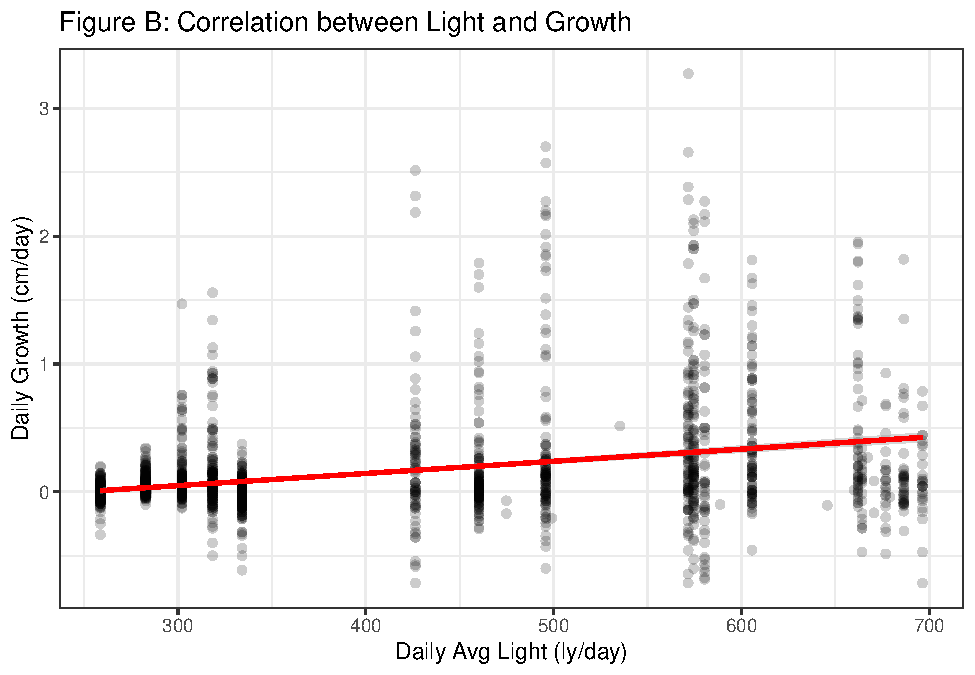
\includegraphics[keepaspectratio]{WK11_2022_23_files/figure-latex/unnamed-chunk-7-1.pdf}}

\emph{Process data}

\begin{Shaded}
\begin{Highlighting}[]
\CommentTok{\#Standardization}
\NormalTok{pl\_lt}\SpecialCharTok{$}\NormalTok{mean\_light\_ly\_day2 }\OtherTok{\textless{}{-}} \FunctionTok{scale}\NormalTok{(pl\_lt}\SpecialCharTok{$}\NormalTok{mean\_light\_ly\_day, }\AttributeTok{center =} \ConstantTok{TRUE}\NormalTok{, }\AttributeTok{scale =} \ConstantTok{TRUE}\NormalTok{)}
\NormalTok{mean\_lt }\OtherTok{\textless{}{-}} \FunctionTok{mean}\NormalTok{(pl\_lt}\SpecialCharTok{$}\NormalTok{mean\_light\_ly\_day, }\AttributeTok{na.rm =} \ConstantTok{TRUE}\NormalTok{)}
\NormalTok{sd\_lt   }\OtherTok{\textless{}{-}} \FunctionTok{sd}\NormalTok{(pl\_lt}\SpecialCharTok{$}\NormalTok{mean\_light\_ly\_day, }\AttributeTok{na.rm =} \ConstantTok{TRUE}\NormalTok{)}

\CommentTok{\#Change Data type}
\NormalTok{pl\_lt }\OtherTok{\textless{}{-}}\NormalTok{ pl\_lt }\SpecialCharTok{\%\textgreater{}\%}
  \FunctionTok{mutate}\NormalTok{(}
    \AttributeTok{pop =} \FunctionTok{factor}\NormalTok{(pop),}
    \AttributeTok{PID        =} \FunctionTok{factor}\NormalTok{(PID),}
    \AttributeTok{block      =} \FunctionTok{factor}\NormalTok{(block)}
\NormalTok{  )}
\end{Highlighting}
\end{Shaded}

\emph{use mixed-effect model to fit relationship between plant growth
and light radiation with population as random effect} \#Q: Does daily
solar radiation positively affect daily growth rate across all
populations? \#Test: Fit a mixed-effect model with population as a
random slope.

\begin{Shaded}
\begin{Highlighting}[]
\NormalTok{pl\_lt.lmer }\OtherTok{\textless{}{-}} \FunctionTok{lmer}\NormalTok{(}
\NormalTok{  daily\_growth }\SpecialCharTok{\textasciitilde{}}\NormalTok{ mean\_light\_ly\_day2 }\SpecialCharTok{+}                     
\NormalTok{    (}\DecValTok{1} \SpecialCharTok{+}\NormalTok{ mean\_light\_ly\_day2 }\SpecialCharTok{|}\NormalTok{ pop),                                    }
  \AttributeTok{data =}\NormalTok{ pl\_lt, }\AttributeTok{REML =} \ConstantTok{TRUE}
\NormalTok{)}
\FunctionTok{summary}\NormalTok{(pl\_lt.lmer)}
\end{Highlighting}
\end{Shaded}

\begin{verbatim}
## Linear mixed model fit by REML ['lmerMod']
## Formula: daily_growth ~ mean_light_ly_day2 + (1 + mean_light_ly_day2 |  
##     pop)
##    Data: pl_lt
## 
## REML criterion at convergence: 1656
## 
## Scaled residuals: 
##     Min      1Q  Median      3Q     Max 
## -4.1389 -0.2891 -0.0481  0.1374  8.6048 
## 
## Random effects:
##  Groups   Name               Variance Std.Dev. Corr
##  pop      (Intercept)        0.02193  0.14807      
##           mean_light_ly_day2 0.00437  0.06611  0.97
##  Residual                    0.11366  0.33713      
## Number of obs: 2415, groups:  pop, 23
## 
## Fixed effects:
##                    Estimate Std. Error t value
## (Intercept)         0.13632    0.03902   3.494
## mean_light_ly_day2  0.07966    0.01999   3.986
## 
## Correlation of Fixed Effects:
##             (Intr)
## mn_lght_l_2 0.916
\end{verbatim}

\emph{overall effect of solar radiation on plant daily growth} \#Figure
C: Relationship between daily average solar radiation and predicted
daily growth rate (cm/day), aggregated across all populations. Each
hexagon represents the density of observations. The black line shows the
fitted regression slope .

\begin{Shaded}
\begin{Highlighting}[]
\CommentTok{\#Unscaling}
\NormalTok{pred\_all }\OtherTok{\textless{}{-}} \FunctionTok{ggpredict}\NormalTok{(pl\_lt.lmer, }\AttributeTok{terms =} \StringTok{"mean\_light\_ly\_day2"}\NormalTok{) }\SpecialCharTok{\%\textgreater{}\%}
  \FunctionTok{as.data.frame}\NormalTok{() }\SpecialCharTok{\%\textgreater{}\%}
  \FunctionTok{mutate}\NormalTok{(}\AttributeTok{light\_orig =}\NormalTok{ x }\SpecialCharTok{*}\NormalTok{ sd\_lt }\SpecialCharTok{+}\NormalTok{ mean\_lt)}

\CommentTok{\#Plot}
\NormalTok{p\_overall }\OtherTok{\textless{}{-}} \FunctionTok{ggplot}\NormalTok{() }\SpecialCharTok{+}
  \FunctionTok{geom\_hex}\NormalTok{(}\AttributeTok{data =}\NormalTok{ pl\_lt,}
           \FunctionTok{aes}\NormalTok{(}\AttributeTok{x =}\NormalTok{ mean\_light\_ly\_day, }\AttributeTok{y =}\NormalTok{ daily\_growth), }\AttributeTok{bins =} \DecValTok{35}\NormalTok{) }\SpecialCharTok{+}
  \FunctionTok{scale\_fill\_viridis\_c}\NormalTok{(}\AttributeTok{name =} \StringTok{"Count"}\NormalTok{) }\SpecialCharTok{+}
  \FunctionTok{geom\_ribbon}\NormalTok{(}\AttributeTok{data =}\NormalTok{ pred\_all,}
              \FunctionTok{aes}\NormalTok{(}\AttributeTok{x =}\NormalTok{ light\_orig, }\AttributeTok{ymin =}\NormalTok{ conf.low, }\AttributeTok{ymax =}\NormalTok{ conf.high),}
              \AttributeTok{alpha =}\NormalTok{ .}\DecValTok{22}\NormalTok{, }\AttributeTok{fill =} \StringTok{"grey60"}\NormalTok{) }\SpecialCharTok{+}
  \FunctionTok{geom\_line}\NormalTok{(}\AttributeTok{data =}\NormalTok{ pred\_all,}
            \FunctionTok{aes}\NormalTok{(}\AttributeTok{x =}\NormalTok{ light\_orig, }\AttributeTok{y =}\NormalTok{ predicted), }\AttributeTok{linewidth =} \DecValTok{1}\NormalTok{) }\SpecialCharTok{+}
  \FunctionTok{labs}\NormalTok{(}\AttributeTok{title =} \StringTok{"Figure C: Effect of Daily Light on Daily Growth (overall)"}\NormalTok{,}
       \AttributeTok{x =} \StringTok{"Daily Avg Light (ly/day)"}\NormalTok{,}
       \AttributeTok{y =} \StringTok{"Predicted Daily Growth (cm/day)"}\NormalTok{) }\SpecialCharTok{+}
  \FunctionTok{theme\_bw}\NormalTok{() }\SpecialCharTok{+}
  \FunctionTok{theme}\NormalTok{(}\AttributeTok{panel.grid.minor =} \FunctionTok{element\_blank}\NormalTok{())}
\NormalTok{p\_overall}
\end{Highlighting}
\end{Shaded}

\begin{verbatim}
## Warning: Removed 11176 rows containing non-finite outside the scale range
## (`stat_binhex()`).
\end{verbatim}

\pandocbounded{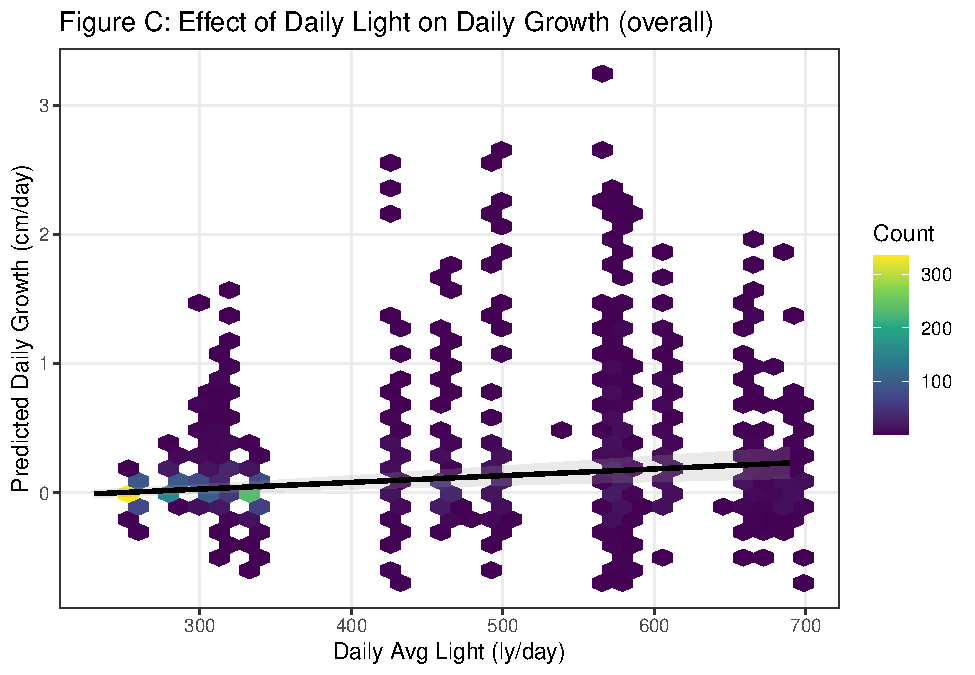
\includegraphics[keepaspectratio]{WK11_2022_23_files/figure-latex/unnamed-chunk-10-1.pdf}}

\emph{Effect of solar radiation on plant daily growth by population}
\#Q: Do different populations vary in their growth response to daily
solar radiation? \#Test: For visualization, scatter plots with fitted
regression lines were drawn separately for each population. \#Figure D:
Light--growth relationship by population. \#Scatter plots show daily
growth rate (cm/day) against daily average solar radiation (ly/day) for
22 populations. Each panel corresponds to one population, with the blue
line indicating the fitted linear trend.

\begin{Shaded}
\begin{Highlighting}[]
\NormalTok{p\_facet }\OtherTok{\textless{}{-}} \FunctionTok{ggplot}\NormalTok{(pl\_lt,}
                  \FunctionTok{aes}\NormalTok{(mean\_light\_ly\_day, daily\_growth)) }\SpecialCharTok{+}
  \FunctionTok{facet\_wrap}\NormalTok{(}\SpecialCharTok{\textasciitilde{}}\NormalTok{ pop, }\AttributeTok{ncol =} \DecValTok{6}\NormalTok{) }\SpecialCharTok{+}
  \FunctionTok{geom\_point}\NormalTok{(}\AttributeTok{alpha =}\NormalTok{ .}\DecValTok{15}\NormalTok{, }\AttributeTok{size =}\NormalTok{ .}\DecValTok{6}\NormalTok{, }\AttributeTok{color =} \StringTok{"grey35"}\NormalTok{) }\SpecialCharTok{+}
  \FunctionTok{geom\_smooth}\NormalTok{(}\AttributeTok{method =} \StringTok{"lm"}\NormalTok{, }\AttributeTok{se =} \ConstantTok{FALSE}\NormalTok{, }\AttributeTok{linewidth =}\NormalTok{ .}\DecValTok{8}\NormalTok{) }\SpecialCharTok{+}
  \FunctionTok{labs}\NormalTok{(}\AttributeTok{title =} \StringTok{"Figure D: Light–Growth relationship by population"}\NormalTok{,}
       \AttributeTok{x =} \StringTok{"Daily Avg Light (ly/day)"}\NormalTok{,}
       \AttributeTok{y =} \StringTok{"Daily Growth (cm/day)"}\NormalTok{) }\SpecialCharTok{+}
  \FunctionTok{theme\_bw}\NormalTok{() }\SpecialCharTok{+}
  \FunctionTok{theme}\NormalTok{(}\AttributeTok{strip.background =} \FunctionTok{element\_rect}\NormalTok{(}\AttributeTok{fill =} \StringTok{"grey95"}\NormalTok{, }\AttributeTok{color =} \ConstantTok{NA}\NormalTok{),}
        \AttributeTok{strip.text =} \FunctionTok{element\_text}\NormalTok{(}\AttributeTok{face =} \StringTok{"bold"}\NormalTok{),}
        \AttributeTok{panel.grid.minor =} \FunctionTok{element\_blank}\NormalTok{())}
\NormalTok{p\_facet}
\end{Highlighting}
\end{Shaded}

\begin{verbatim}
## `geom_smooth()` using formula = 'y ~ x'
\end{verbatim}

\begin{verbatim}
## Warning: Removed 11176 rows containing non-finite outside the scale range
## (`stat_smooth()`).
\end{verbatim}

\begin{verbatim}
## Warning: Removed 11176 rows containing missing values or values outside the scale range
## (`geom_point()`).
\end{verbatim}

\pandocbounded{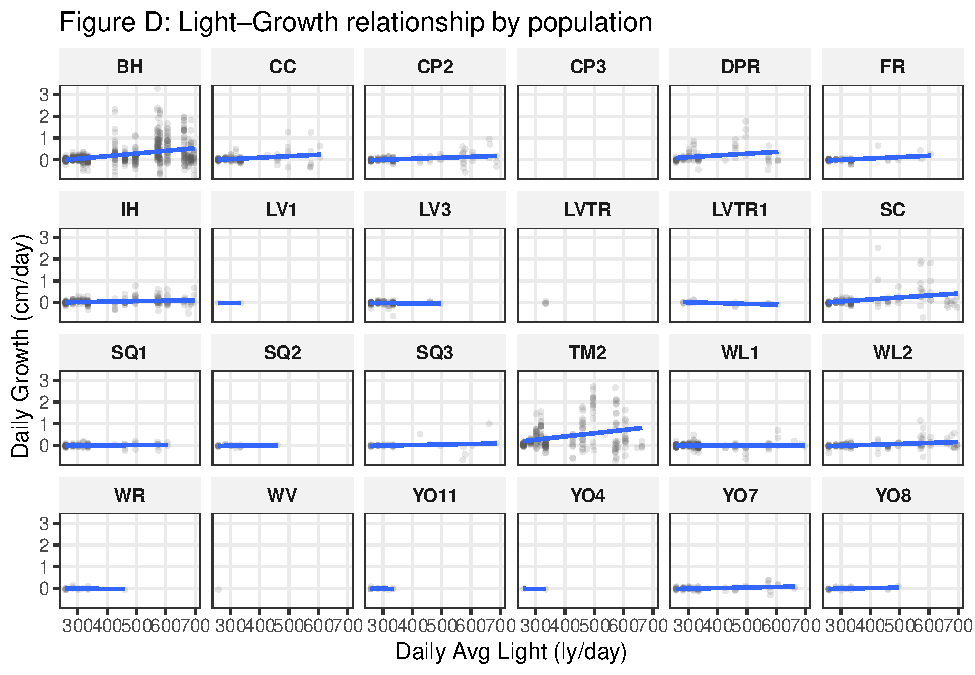
\includegraphics[keepaspectratio]{WK11_2022_23_files/figure-latex/unnamed-chunk-11-1.pdf}}

\emph{Find slope of plant growth and solar radiation for each
population} \#Q: Which populations show significantly positive or
negligible slopes in the light--growth relationship? \#Method: Extract
slopes and 95\% confidence intervals for each population from the
mixed-effects model \#Figure E. Population-specific slopes with 95\%
confidence intervals. \#The slope of the light--growth relationship
(cm/day per Ly/day) is shown for each population. Points indicate
estimated slopes and horizontal lines show 95\% CIs. The vertical dashed
line marks zero effect. Most populations exhibit positive slopes,
suggesting that higher solar radiation is generally associated with
faster daily growth, although the strength and significance of this
relationship vary across populations.

\begin{Shaded}
\begin{Highlighting}[]
\CommentTok{\#slope and standard deviation of fixed effects}
\NormalTok{b\_fix  }\OtherTok{\textless{}{-}} \FunctionTok{fixef}\NormalTok{(pl\_lt.lmer)[}\StringTok{"mean\_light\_ly\_day2"}\NormalTok{]}
\NormalTok{V\_fix  }\OtherTok{\textless{}{-}} \FunctionTok{vcov}\NormalTok{(pl\_lt.lmer)[}\StringTok{"mean\_light\_ly\_day2"}\NormalTok{,}\StringTok{"mean\_light\_ly\_day2"}\NormalTok{]}

\CommentTok{\#slope and standard deviation of random effects}
\NormalTok{re }\OtherTok{\textless{}{-}} \FunctionTok{ranef}\NormalTok{(pl\_lt.lmer, }\AttributeTok{condVar =} \ConstantTok{TRUE}\NormalTok{) }
\NormalTok{re\_pop }\OtherTok{\textless{}{-}}\NormalTok{ re}\SpecialCharTok{$}\NormalTok{pop}
\NormalTok{postVar }\OtherTok{\textless{}{-}} \FunctionTok{attr}\NormalTok{(re}\SpecialCharTok{$}\NormalTok{pop, }\StringTok{"postVar"}\NormalTok{)           }
\NormalTok{sl\_col }\OtherTok{\textless{}{-}} \FunctionTok{which}\NormalTok{(}\FunctionTok{colnames}\NormalTok{(re\_pop) }\SpecialCharTok{==} \StringTok{"mean\_light\_ly\_day2"}\NormalTok{)}

\CommentTok{\#create the tibble of slopes for each population}
\NormalTok{pop\_slope }\OtherTok{\textless{}{-}} \FunctionTok{tibble}\NormalTok{(}
  \AttributeTok{parent\_pop   =} \FunctionTok{rownames}\NormalTok{(re\_pop),}
  \AttributeTok{rand\_slope   =}\NormalTok{ re\_pop[ , }\StringTok{"mean\_light\_ly\_day2"}\NormalTok{],}
  \AttributeTok{rand\_var     =} \FunctionTok{sapply}\NormalTok{(}\FunctionTok{seq\_len}\NormalTok{(}\FunctionTok{dim}\NormalTok{(postVar)[}\DecValTok{3}\NormalTok{]), }\ControlFlowTok{function}\NormalTok{(i) postVar[sl\_col, sl\_col, i])}
\NormalTok{) }\SpecialCharTok{\%\textgreater{}\%}
  \FunctionTok{mutate}\NormalTok{(}
    \AttributeTok{slope\_SD   =}\NormalTok{ b\_fix }\SpecialCharTok{+}\NormalTok{ rand\_slope,                        }
    \AttributeTok{se\_SD      =} \FunctionTok{sqrt}\NormalTok{(V\_fix }\SpecialCharTok{+}\NormalTok{ rand\_var),               }
    \AttributeTok{lower\_SD   =}\NormalTok{ slope\_SD }\SpecialCharTok{{-}} \FloatTok{1.96}\SpecialCharTok{*}\NormalTok{se\_SD,}
    \AttributeTok{upper\_SD   =}\NormalTok{ slope\_SD }\SpecialCharTok{+} \FloatTok{1.96}\SpecialCharTok{*}\NormalTok{se\_SD}
\NormalTok{  )}

\NormalTok{pop\_slope }\OtherTok{\textless{}{-}}\NormalTok{ pop\_slope }\SpecialCharTok{\%\textgreater{}\%}
  \FunctionTok{mutate}\NormalTok{(}
    \AttributeTok{slope\_per\_Wm2 =}\NormalTok{ slope\_SD }\SpecialCharTok{/}\NormalTok{ sd\_lt,}
    \AttributeTok{lower\_per\_Wm2 =}\NormalTok{ lower\_SD }\SpecialCharTok{/}\NormalTok{ sd\_lt,}
    \AttributeTok{upper\_per\_Wm2 =}\NormalTok{ upper\_SD }\SpecialCharTok{/}\NormalTok{ sd\_lt}
\NormalTok{  )}\SpecialCharTok{\%\textgreater{}\%}
  \FunctionTok{select}\NormalTok{(parent\_pop, slope\_per\_Wm2, lower\_per\_Wm2, upper\_per\_Wm2)}
\NormalTok{pop\_slope}
\end{Highlighting}
\end{Shaded}

\begin{verbatim}
## # A tibble: 23 x 4
##    parent_pop slope_per_Wm2 lower_per_Wm2 upper_per_Wm2
##    <chr>              <dbl>         <dbl>         <dbl>
##  1 BH              0.00113      0.000837       0.00142 
##  2 CC              0.000595     0.000124       0.00106 
##  3 CP2             0.000425     0.0000137      0.000835
##  4 DPR             0.000889     0.000429       0.00135 
##  5 FR              0.000462    -0.0000947      0.00102 
##  6 IH              0.000307    -0.0000424      0.000656
##  7 LV1             0.000503    -0.000362       0.00137 
##  8 LV3             0.000251    -0.000328       0.000830
##  9 LVTR            0.000481    -0.000347       0.00131 
## 10 LVTR1           0.000208    -0.000393       0.000808
## # i 13 more rows
\end{verbatim}

\begin{Shaded}
\begin{Highlighting}[]
\FunctionTok{write.csv}\NormalTok{(pop\_slope, }\StringTok{"population\_slopes.csv"}\NormalTok{, }\AttributeTok{row.names =} \ConstantTok{FALSE}\NormalTok{)}

\CommentTok{\#plot}
\FunctionTok{ggplot}\NormalTok{(pop\_slope, }\FunctionTok{aes}\NormalTok{(}\AttributeTok{x =} \FunctionTok{reorder}\NormalTok{(parent\_pop, slope\_per\_Wm2), }\AttributeTok{y =}\NormalTok{ slope\_per\_Wm2)) }\SpecialCharTok{+}
  \FunctionTok{geom\_hline}\NormalTok{(}\AttributeTok{yintercept =} \DecValTok{0}\NormalTok{, }\AttributeTok{linetype =} \DecValTok{2}\NormalTok{) }\SpecialCharTok{+}
  \FunctionTok{geom\_pointrange}\NormalTok{(}\FunctionTok{aes}\NormalTok{(}\AttributeTok{ymin =}\NormalTok{ lower\_per\_Wm2, }\AttributeTok{ymax =}\NormalTok{ upper\_per\_Wm2), }\AttributeTok{linewidth =}\NormalTok{ .}\DecValTok{6}\NormalTok{) }\SpecialCharTok{+}
  \FunctionTok{coord\_flip}\NormalTok{() }\SpecialCharTok{+}
  \FunctionTok{labs}\NormalTok{(}\AttributeTok{title =} \StringTok{"Figure E: Population{-}specific slopes with 95\% CI"}\NormalTok{,}
       \AttributeTok{x =} \StringTok{"Population"}\NormalTok{, }\AttributeTok{y =} \StringTok{"Slope (cm/day per ly/day)"}\NormalTok{) }\SpecialCharTok{+}
  \FunctionTok{theme\_bw}\NormalTok{()}
\end{Highlighting}
\end{Shaded}

\pandocbounded{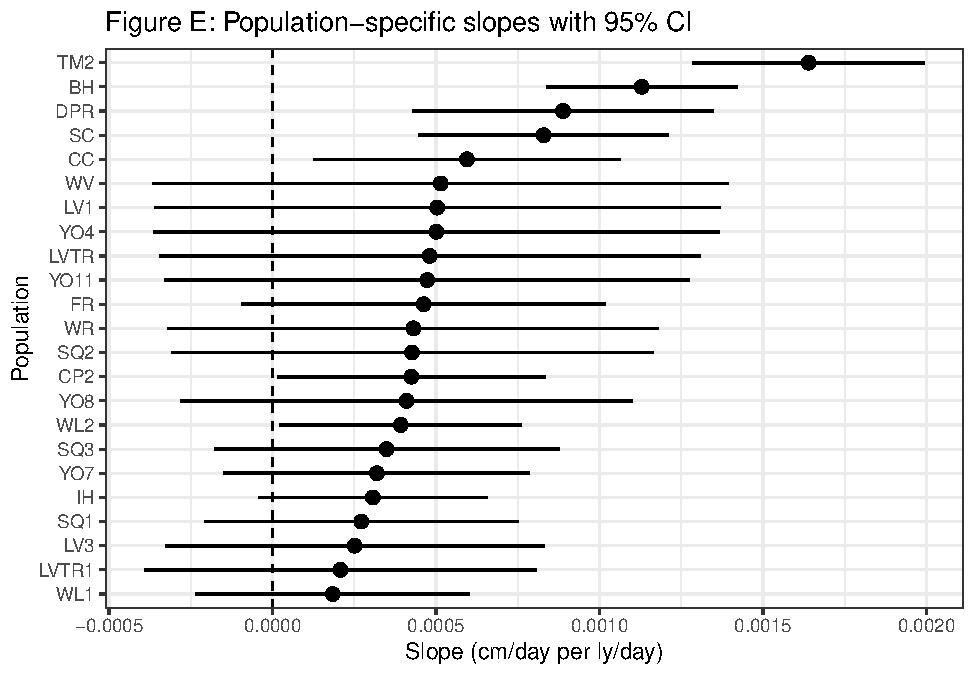
\includegraphics[keepaspectratio]{WK11_2022_23_files/figure-latex/unnamed-chunk-12-1.pdf}}

\emph{height\_time plot with solar radiation as color}

\begin{Shaded}
\begin{Highlighting}[]
\NormalTok{pl\_lt}\SpecialCharTok{\%\textgreater{}\%}
  \FunctionTok{ggplot}\NormalTok{(}\FunctionTok{aes}\NormalTok{(survey\_date, height, }\AttributeTok{colour =}\NormalTok{ mean\_light\_ly\_day, }\AttributeTok{group=}\NormalTok{PID)) }\SpecialCharTok{+}
  \FunctionTok{facet\_wrap}\NormalTok{(}\SpecialCharTok{\textasciitilde{}}\NormalTok{pop)}\SpecialCharTok{+}
  \FunctionTok{scale\_colour\_gradientn}\NormalTok{(                         }\CommentTok{\# low=blue, high=red}
    \AttributeTok{colours =} \FunctionTok{c}\NormalTok{(}\StringTok{"\#2c7bb6"}\NormalTok{,}\StringTok{"\#abd9e9"}\NormalTok{,}\StringTok{"\#ffffbf"}\NormalTok{,}\StringTok{"\#fdae61"}\NormalTok{,}\StringTok{"\#d7191c"}\NormalTok{),}
    \AttributeTok{name =} \StringTok{"Solar Radiation (W/m²)"}\NormalTok{)}\SpecialCharTok{+}
  \FunctionTok{geom\_point}\NormalTok{(}\AttributeTok{alpha=}\FloatTok{0.25}\NormalTok{,}\AttributeTok{size=}\FloatTok{0.5}\NormalTok{)}\SpecialCharTok{+}
  \FunctionTok{geom\_line}\NormalTok{(}\AttributeTok{alpha=}\FloatTok{0.5}\NormalTok{) }\SpecialCharTok{+}
  \FunctionTok{scale\_x\_date}\NormalTok{(}\AttributeTok{date\_breaks =} \StringTok{"1 month"}\NormalTok{, }\AttributeTok{date\_labels =} \StringTok{"\%b"}\NormalTok{) }\SpecialCharTok{+}
   \FunctionTok{scale\_y\_continuous}\NormalTok{(}
    \AttributeTok{name =} \StringTok{"Height (cm)"}\NormalTok{)}\SpecialCharTok{+}
  \FunctionTok{labs}\NormalTok{(}\AttributeTok{title =} \StringTok{"Figure F.1: Time{-}Height"}\NormalTok{,}
       \AttributeTok{x =} \StringTok{"Survey Date"}\NormalTok{,}
       \AttributeTok{y =} \StringTok{"Height (cm)"}\NormalTok{) }\SpecialCharTok{+}
  \FunctionTok{guides}\NormalTok{(}\AttributeTok{x =} \FunctionTok{guide\_axis}\NormalTok{(}\AttributeTok{n.dodge =} \DecValTok{2}\NormalTok{))}\SpecialCharTok{+}
  \FunctionTok{theme\_bw}\NormalTok{()}\SpecialCharTok{+}
  \FunctionTok{theme}\NormalTok{(}\AttributeTok{axis.text.x =} \FunctionTok{element\_text}\NormalTok{(}\AttributeTok{angle=}\DecValTok{30}\NormalTok{))}
\end{Highlighting}
\end{Shaded}

\begin{verbatim}
## Warning: Removed 10542 rows containing missing values or values outside the scale range
## (`geom_point()`).
\end{verbatim}

\begin{verbatim}
## Warning: Removed 10533 rows containing missing values or values outside the scale range
## (`geom_line()`).
\end{verbatim}

\begin{verbatim}
## `geom_line()`: Each group consists of only one observation.
## i Do you need to adjust the group aesthetic?
\end{verbatim}

\pandocbounded{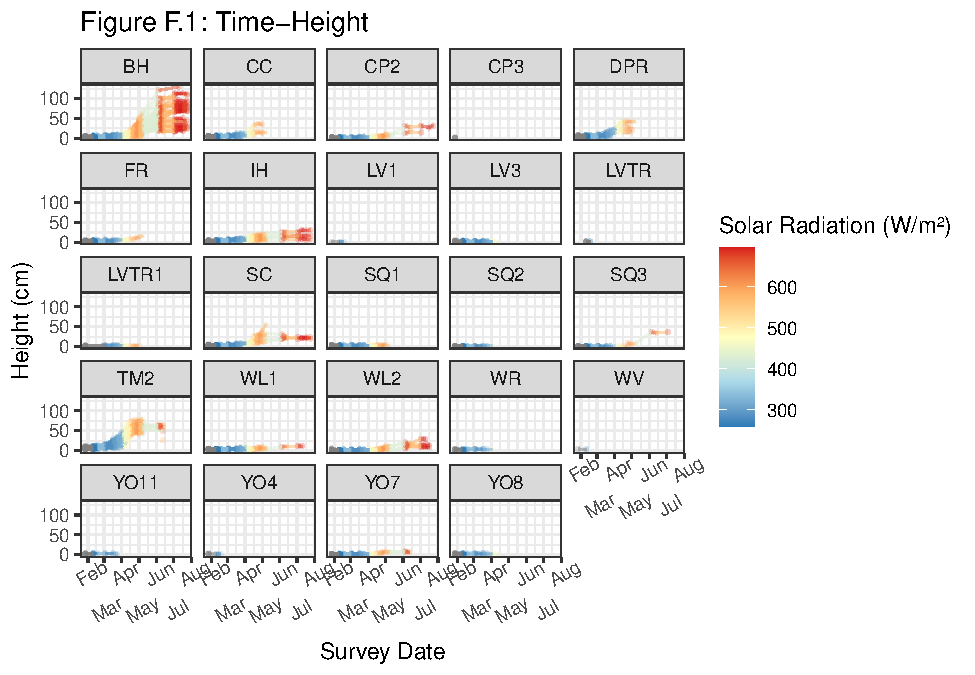
\includegraphics[keepaspectratio]{WK11_2022_23_files/figure-latex/unnamed-chunk-13-1.pdf}}

\begin{Shaded}
\begin{Highlighting}[]
\NormalTok{pl\_lt}\SpecialCharTok{\%\textgreater{}\%}
  \FunctionTok{filter}\NormalTok{(pop}\SpecialCharTok{==}\StringTok{"TM2"}\NormalTok{)}\SpecialCharTok{\%\textgreater{}\%}
  \FunctionTok{ggplot}\NormalTok{(}\FunctionTok{aes}\NormalTok{(survey\_date, height, }\AttributeTok{colour =}\NormalTok{ mean\_light\_ly\_day, }\AttributeTok{group=}\NormalTok{PID)) }\SpecialCharTok{+}
  \FunctionTok{scale\_colour\_gradientn}\NormalTok{(                         }\CommentTok{\# low=blue, high=red}
    \AttributeTok{colours =} \FunctionTok{c}\NormalTok{(}\StringTok{"\#2c7bb6"}\NormalTok{,}\StringTok{"\#abd9e9"}\NormalTok{,}\StringTok{"\#ffffbf"}\NormalTok{,}\StringTok{"\#fdae61"}\NormalTok{,}\StringTok{"\#d7191c"}\NormalTok{),}
    \AttributeTok{name =} \StringTok{"Solar Radiation (W/m²)"}\NormalTok{)}\SpecialCharTok{+}
  \FunctionTok{geom\_point}\NormalTok{(}\AttributeTok{alpha=}\DecValTok{1}\NormalTok{,}\AttributeTok{size=}\FloatTok{0.5}\NormalTok{)}\SpecialCharTok{+}
  \FunctionTok{geom\_line}\NormalTok{(}\AttributeTok{alpha=}\DecValTok{1}\NormalTok{) }\SpecialCharTok{+}
  \FunctionTok{scale\_x\_date}\NormalTok{(}\AttributeTok{date\_breaks =} \StringTok{"1 month"}\NormalTok{, }\AttributeTok{date\_labels =} \StringTok{"\%b"}\NormalTok{) }\SpecialCharTok{+}
   \FunctionTok{scale\_y\_continuous}\NormalTok{(}
    \AttributeTok{name =} \StringTok{"Height (cm)"}\NormalTok{)}\SpecialCharTok{+}
  \FunctionTok{labs}\NormalTok{(}\AttributeTok{title =} \StringTok{"Figure F.2: Time{-}Height for TM2"}\NormalTok{,}
       \AttributeTok{x =} \StringTok{"Survey Date"}\NormalTok{,}
       \AttributeTok{y =} \StringTok{"Height (cm)"}\NormalTok{) }\SpecialCharTok{+}
  \FunctionTok{theme\_bw}\NormalTok{()}
\end{Highlighting}
\end{Shaded}

\begin{verbatim}
## Warning: Removed 379 rows containing missing values or values outside the scale range
## (`geom_point()`).
\end{verbatim}

\begin{verbatim}
## Warning: Removed 377 rows containing missing values or values outside the scale range
## (`geom_line()`).
\end{verbatim}

\pandocbounded{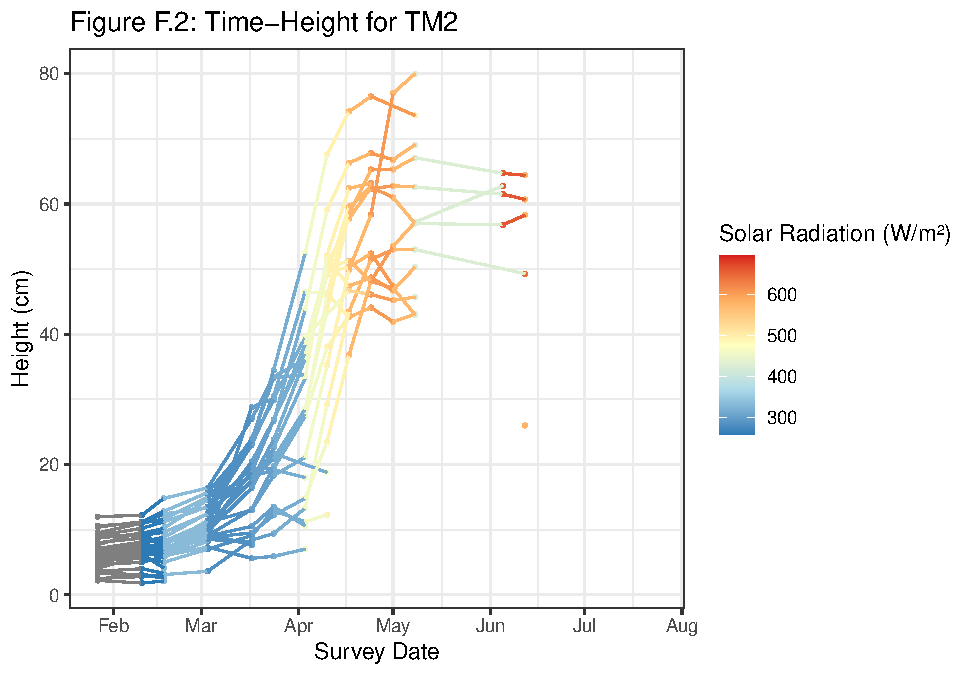
\includegraphics[keepaspectratio]{WK11_2022_23_files/figure-latex/unnamed-chunk-14-1.pdf}}

\begin{Shaded}
\begin{Highlighting}[]
\NormalTok{pl\_lt}\SpecialCharTok{\%\textgreater{}\%}
  \FunctionTok{filter}\NormalTok{(pop}\SpecialCharTok{==}\StringTok{"BH"}\NormalTok{)}\SpecialCharTok{\%\textgreater{}\%}
  \FunctionTok{ggplot}\NormalTok{(}\FunctionTok{aes}\NormalTok{(survey\_date, height, }\AttributeTok{colour =}\NormalTok{ mean\_light\_ly\_day, }\AttributeTok{group=}\NormalTok{PID)) }\SpecialCharTok{+}
  \FunctionTok{scale\_colour\_gradientn}\NormalTok{(                         }\CommentTok{\# low=blue, high=red}
    \AttributeTok{colours =} \FunctionTok{c}\NormalTok{(}\StringTok{"\#2c7bb6"}\NormalTok{,}\StringTok{"\#abd9e9"}\NormalTok{,}\StringTok{"\#ffffbf"}\NormalTok{,}\StringTok{"\#fdae61"}\NormalTok{,}\StringTok{"\#d7191c"}\NormalTok{),}
    \AttributeTok{name =} \StringTok{"Solar Radiation (W/m²)"}\NormalTok{)}\SpecialCharTok{+}
  \FunctionTok{geom\_point}\NormalTok{(}\AttributeTok{alpha=}\DecValTok{1}\NormalTok{,}\AttributeTok{size=}\FloatTok{0.5}\NormalTok{)}\SpecialCharTok{+}
  \FunctionTok{geom\_line}\NormalTok{(}\AttributeTok{alpha=}\DecValTok{1}\NormalTok{) }\SpecialCharTok{+}
  \FunctionTok{scale\_x\_date}\NormalTok{(}\AttributeTok{date\_breaks =} \StringTok{"1 month"}\NormalTok{, }\AttributeTok{date\_labels =} \StringTok{"\%b"}\NormalTok{) }\SpecialCharTok{+}
   \FunctionTok{scale\_y\_continuous}\NormalTok{(}
    \AttributeTok{name =} \StringTok{"Height (cm)"}\NormalTok{)}\SpecialCharTok{+}
  \FunctionTok{labs}\NormalTok{(}\AttributeTok{title =} \StringTok{"Figure F.3: Time{-}Height for BH"}\NormalTok{,}
       \AttributeTok{x =} \StringTok{"Survey Date"}\NormalTok{,}
       \AttributeTok{y =} \StringTok{"Height (cm)"}\NormalTok{) }\SpecialCharTok{+}
  \FunctionTok{theme\_bw}\NormalTok{()}
\end{Highlighting}
\end{Shaded}

\begin{verbatim}
## Warning: Removed 1176 rows containing missing values or values outside the scale range
## (`geom_point()`).
\end{verbatim}

\begin{verbatim}
## Warning: Removed 1174 rows containing missing values or values outside the scale range
## (`geom_line()`).
\end{verbatim}

\pandocbounded{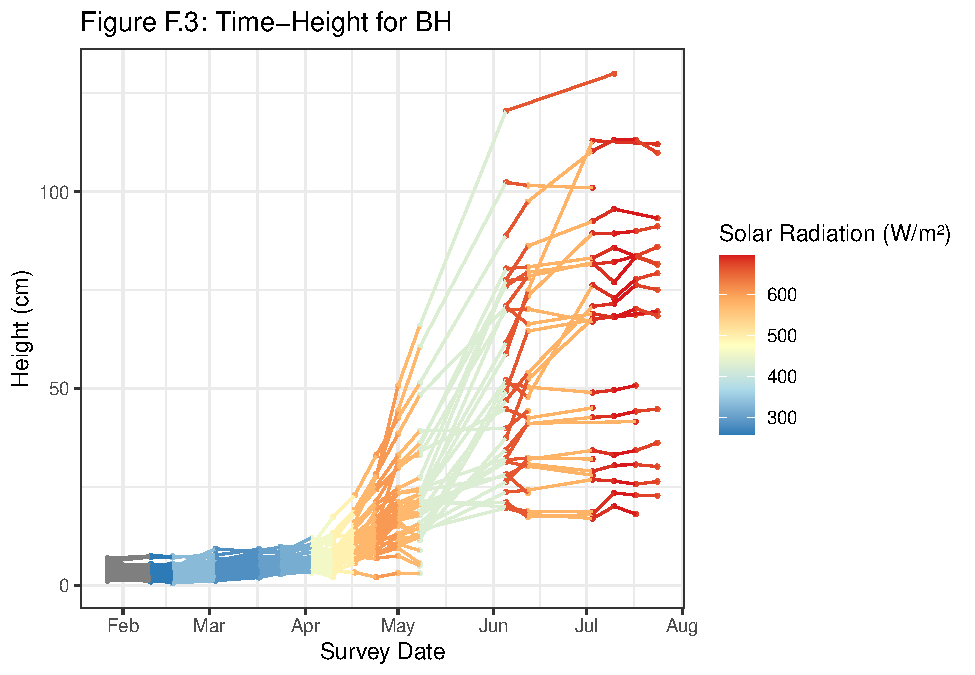
\includegraphics[keepaspectratio]{WK11_2022_23_files/figure-latex/unnamed-chunk-15-1.pdf}}

\begin{Shaded}
\begin{Highlighting}[]
\NormalTok{pl\_lt}\SpecialCharTok{\%\textgreater{}\%}
  \FunctionTok{filter}\NormalTok{(pop}\SpecialCharTok{==}\StringTok{"DPR"}\NormalTok{)}\SpecialCharTok{\%\textgreater{}\%}
  \FunctionTok{ggplot}\NormalTok{(}\FunctionTok{aes}\NormalTok{(survey\_date, height, }\AttributeTok{colour =}\NormalTok{ mean\_light\_ly\_day, }\AttributeTok{group=}\NormalTok{PID)) }\SpecialCharTok{+}
  \FunctionTok{scale\_colour\_gradientn}\NormalTok{(                         }\CommentTok{\# low=blue, high=red}
    \AttributeTok{colours =} \FunctionTok{c}\NormalTok{(}\StringTok{"\#2c7bb6"}\NormalTok{,}\StringTok{"\#abd9e9"}\NormalTok{,}\StringTok{"\#ffffbf"}\NormalTok{,}\StringTok{"\#fdae61"}\NormalTok{,}\StringTok{"\#d7191c"}\NormalTok{),}
    \AttributeTok{name =} \StringTok{"Solar Radiation (W/m²)"}\NormalTok{)}\SpecialCharTok{+}
  \FunctionTok{geom\_point}\NormalTok{(}\AttributeTok{alpha=}\DecValTok{1}\NormalTok{,}\AttributeTok{size=}\FloatTok{0.5}\NormalTok{)}\SpecialCharTok{+}
  \FunctionTok{geom\_line}\NormalTok{(}\AttributeTok{alpha=}\DecValTok{1}\NormalTok{) }\SpecialCharTok{+}
  \FunctionTok{scale\_x\_date}\NormalTok{(}\AttributeTok{date\_breaks =} \StringTok{"1 month"}\NormalTok{, }\AttributeTok{date\_labels =} \StringTok{"\%b"}\NormalTok{) }\SpecialCharTok{+}
   \FunctionTok{scale\_y\_continuous}\NormalTok{(}
    \AttributeTok{name =} \StringTok{"Height (cm)"}\NormalTok{)}\SpecialCharTok{+}
  \FunctionTok{labs}\NormalTok{(}\AttributeTok{title =} \StringTok{"Figure F.4: Time{-}Height for DPR"}\NormalTok{,}
       \AttributeTok{x =} \StringTok{"Survey Date"}\NormalTok{,}
       \AttributeTok{y =} \StringTok{"Height (cm)"}\NormalTok{) }\SpecialCharTok{+}
  \FunctionTok{theme\_bw}\NormalTok{()}
\end{Highlighting}
\end{Shaded}

\begin{verbatim}
## Warning: Removed 291 rows containing missing values or values outside the scale range
## (`geom_point()`).
\end{verbatim}

\begin{verbatim}
## Warning: Removed 291 rows containing missing values or values outside the scale range
## (`geom_line()`).
\end{verbatim}

\pandocbounded{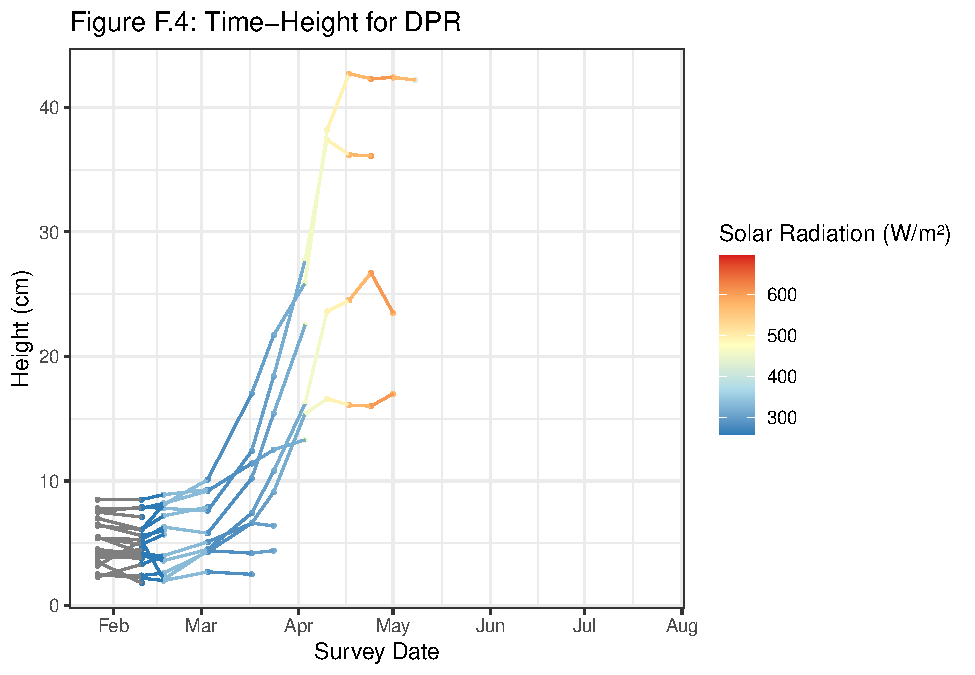
\includegraphics[keepaspectratio]{WK11_2022_23_files/figure-latex/unnamed-chunk-16-1.pdf}}

\end{document}
